\section{Обзор современных подходов}
\label{sec:Chapter1} \index{Chapter1}
\subsection{Обучение по нескольким примерам}

Поставим задачу FSL формально:  Пусть $R$ - ожидаемый риск; $\mathcal{H}$ - пространство гипотез; $\hat{h}$ - функция, минимизирующая ожидаемый риск; $h^*$ - функция в $\mathcal{H}$, минимизируящая ожидаемый риск; $h_I$ - функция в $\mathcal{H}$, минимизирующая эмпирический риск. Тогда общую ошибку можно представить в виде \cite{FSLsurvey}:

\large
$$
\mathbb{E}\left[R\left(h_I\right)-R(\hat{h})\right]=\underbrace{\mathbb{E}\left[R\left(h^*\right)-R(\hat{h})\right]}_{\mathcal{E}_{\text {app }}(\mathcal{H})}+\underbrace{\mathbb{E}\left[R\left(h_I\right)-R\left(h^*\right)\right]}_{\mathcal{E}_{\text {est }}(\mathcal{H}, I)}
$$

\normalsize
$\mathcal{E}_{\text {app }}$ - ошибка приближения (approximation), показывающая насколько хорошо могут функции в $\mathcal{H}$ аппроксимировать $\hat{h}$; $\mathcal{E}_{\text {est }}$ - ошибка расчета (estimation) показывает насколько хорошо мы можем приблизиться к $h^*$ в $\mathcal{H}$, минимизируя эмпирический риск.

\begin{figure}[h!]
\caption{Влияние размера обучающей выборки $I$ на $h_I$}
\centering
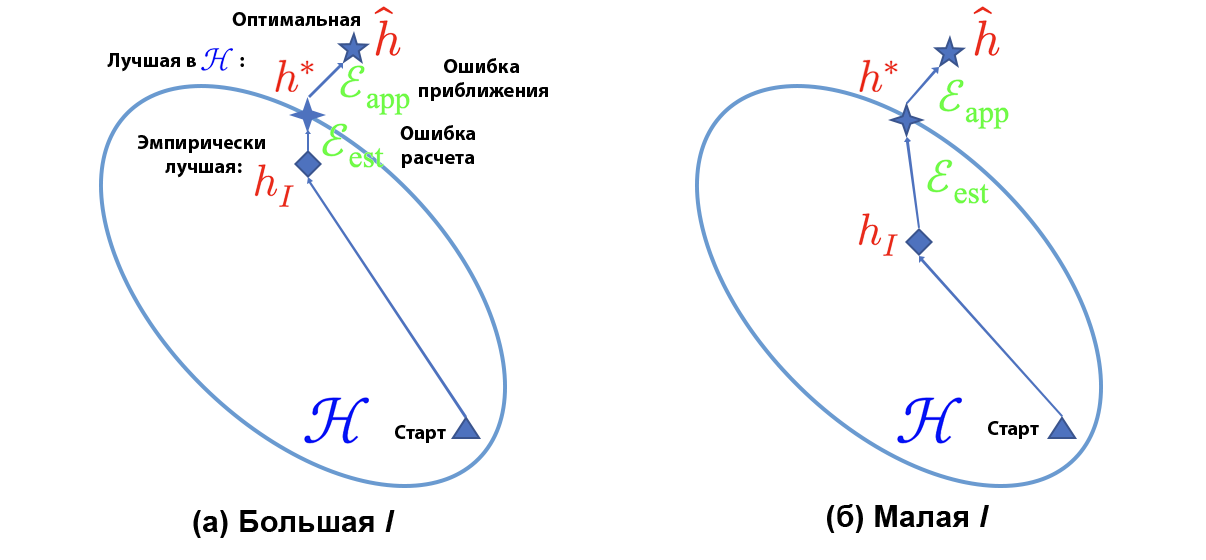
\includegraphics[width=16cm]{Images/H_largesmall_I_rus_noback.png}
\label{fig:H_largesmall_I_rus_noback}
\end{figure}

\begin{figure}[h!]

\centering
\end{figure}

\newpage

Используя некоторые предварительные знания о задаче можно выделить три подхода (Рис. \ref{fig:FSL_taxomony_rus_noback}) к уменьшению $\mathcal{E}_{\text {est }}$ \cite{FSLsurvey}: 
\begin{itemize}
    \item \textbf{Данные}. Увеличение обучающей выборки за счет преобразования объектов заданного датасета \cite{ReviewShareddensities, ReviewDeltaEncoder, ReviewLowShotVisual, ReviewOneShotSceneLocations, ReviewFeatureSpaceTransfer}, использования объектов из неразмеченных \cite{Review, ReviewLowShotDiffusion, ReviewStepwiseLearning}, слаборазмеченных датасетов или похожих датасетов \cite{ReviewStepwiseLearning, ReviewGenerativeAdversalNets, ReviewLowShotAugmentationNets}.
    \item \textbf{Модель}. Упрощение пространства гипотез $\mathcal{H}$. Тогда в новом пространстве $\Tilde{\mathcal{H}}$ имеющейся обучающей выборки будет достаточно для обучения. Различают многозадачное обучение \cite{ReviewMultitaskLearning, ReviewSurveyMultiTask, ReviewDeepLearning}, обучение эмбеддингов \cite{ReviewConvolutionArchitectureEmbedding, ReviewDifferentialGeometry}, обучение с внешней памятью \cite{ReviewNeuralTuringMachines, ReviewKeyValueMemory, ReviewEndToEndMemory,  ReviewMemoryNetworks}  и генеративное моделлирование \cite{ReviewNeuralStatistician, ReviewConceptLearning, ReviewFewShotAutoregressive, ReviewOneShotGeneralization}.
    \item \textbf{Алгоритм}. Выбор хорошей стартовой точки для обучения или добавление дополнительного шага в процессе обучения помимо шага минимизатора эмпирического риска. Выделяют такие методы, как уточнение существующих параметров \cite{ReviewOneShotVideoSegmentation}, уточнение мета-обученных параметров \cite{ReviewMetaLearningFastAdaptation} и обучение оптимизатора \cite{ReviewGradientDescendDouble, ReviewOptimizationModelFewShot}.
\end{itemize}

\begin{figure}[!h]
\caption{Схема подходов в FSL}
\centering
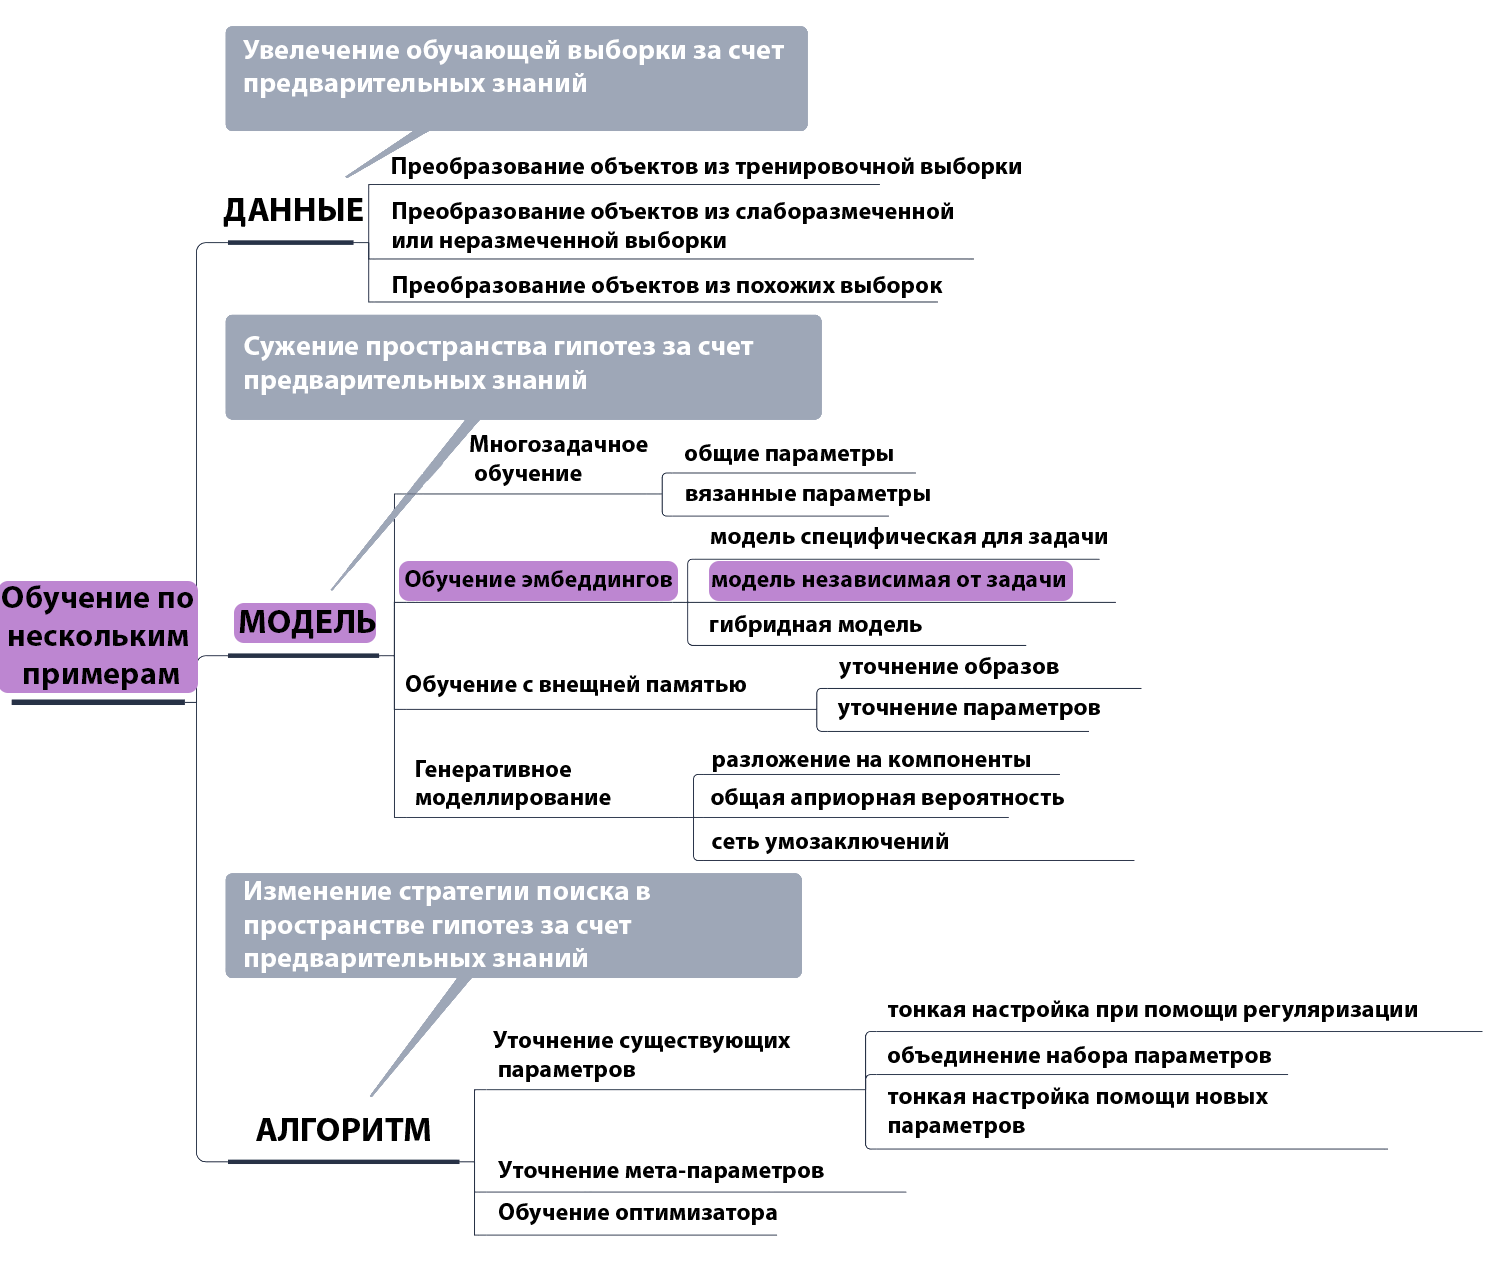
\includegraphics[width=16cm]{Images/FSL_taxomony_rus_noback.png}
\label{fig:FSL_taxomony_rus_noback}
\end{figure}

Легко заметить, что в прикладных задачах могут быть применены различные комбинации подходов или все три одновременно, поскольку они затрагивают разные аспекты обучения. Подробное описание каждого из подходов, изображенных на Рис. \ref{fig:FSL_taxomony_rus_noback} изложено в статье \cite{FSLsurvey}. Тем не менее, поскольку обучение эмбеддингов является неотъемлемой частью данного исследования, ниже изложено более подробное описание этого метода.

\newpage
\subsubsection{Обучение эмбеддингов}

\label{subsec:EmbeddingLearning}

    Суть построения эмбеддингов \cite{ReviewConvolutionArchitectureEmbedding} - перевод объектов из начального пространства ${x_i}\in\mathcal{X}\subset\mathbb{R}^n$ в пространство меньшей размерности ${z_i}\in\mathcal{Z}\subset\mathbb{R}^m, m < n$, в котором уже и производить классификацию. Причем $\mathcal{Z}$ должно быть таким, что похожие примеры должны быть близки друг к другу, а различные - удалены.

    Одним из наиболее простых методов построения сети эмбеддингов является использование части классификатора: сначала строится сеть, классифицирующая на большое число классов, а после удаляется последний слой (слой вывода), оставшаяся часть и есть генератор эмбеддингов (Рис. \ref{fig:embed_from_mlp}).

\begin{figure}[!h]
\caption{Построение генератора эмбеддингов с помощью классификатора}
\centering
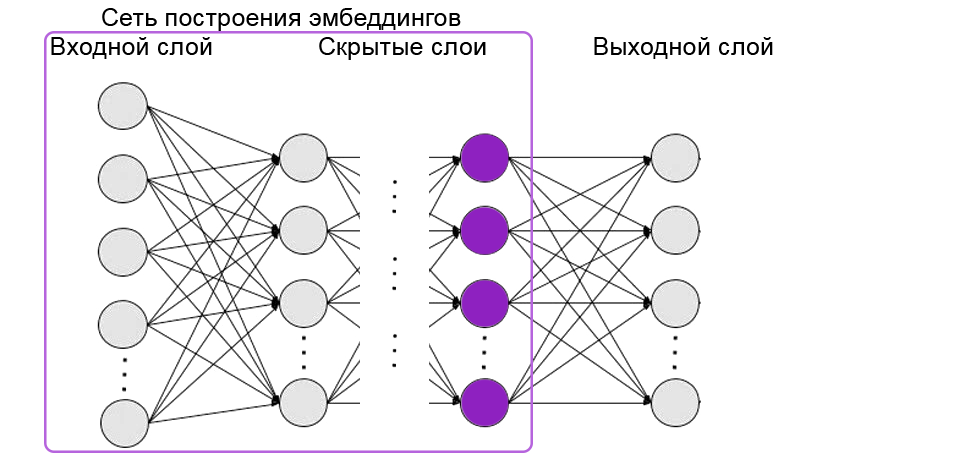
\includegraphics[width=16cm]{Images/embed_from_mlp.png}
\label{fig:embed_from_mlp}
\end{figure}


    Основные компоненты обучения эмбеддингов: функция $f$, переводящая тестовый пример $x_{\text {test }} \in D_{\text {test }}$ в пространство эмбеддингов $\mathcal{Z}$, функция $g$, переводящая объекты из тренировочного датасета $x_i \in D_{\text {train }}$ в $\mathcal{Z}$, функция схожести (расстояния) $s(x_i, x_j)$. Обычно функции $f$ и $g$ совпадают.

    По тому, как меняются параметры функций $f$ и $g$ от задачи к задаче выделяют три метода построения эмбеддингов: индивидуальный для каждой задачи (task-specific), независимый (task-invariant) и гибридный.

\begin{itemize}
    \item \textbf{Task-specific (Специфическая для каждой задачи)} \cite{ReviewEmbedInformationLens}. Обучение проводится только на объектах из обучающей выборки для конкретной задачи. 
    \item \textbf{Task-invariant (Модель, независящая от задачи)} \cite{ReviewEmbedObjectClassification, ReviewSiameseNeuralNetworks} Рис. \ref{fig:FSL_Embedding_general_rus_noback}. Обучение проводится на большой обучающей выборке, а после обученная модель применяется без переобучения для специфической задачи.
    \label{pos:TaskInvariant}
    \item \textbf{Гибридная модель} \cite{ReviewEmbedFeedForward} Рис. \ref{fig:FSL_Embedding_hybrid_rus_noback}. Гибридная модель объединяет в себе предыдущие два подхода: эмбеддинги, полученные при использовании независимой модели, используются как параметр для построения эмбеддингов для конкретной задачи.
\end{itemize}

\begin{figure}[h!]
\caption{Независимая модель построения эмбеддингов}
\centering
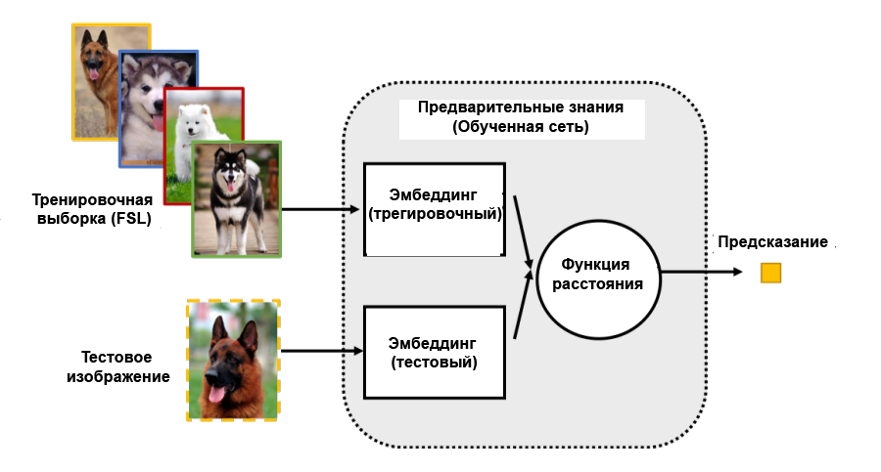
\includegraphics[width=16cm]{Images/FSL_Embedding_general_rus_noback.png}
\label{fig:FSL_Embedding_general_rus_noback}
\end{figure}

\begin{figure}[h!]
\caption{Гибридная модель построения эмбеддингов}
\centering
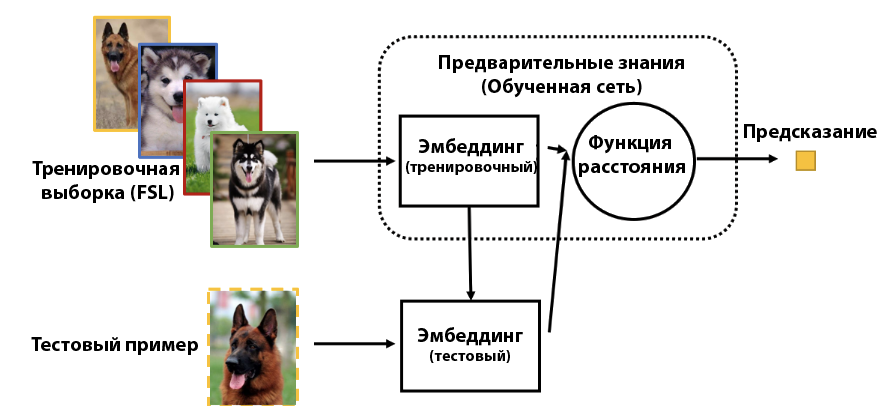
\includegraphics[width=16cm]{Images/FSL_Embedding_hybrid_rus_noback.png}
\label{fig:FSL_Embedding_hybrid_rus_noback}
\end{figure}